\chapter{Бинарные логические операции}

\section{Логическое И}

Как вы уже знаете, реле представляет собой управляемый выключатель или переключатель.
Если на один контакт $A$ выключателя подать сигнал, то на другом $C$ он появится
только если на обмотке реле $B$ есть напряжение (логическая единица).

\begin{center}
\includegraphics{schemes/and.png}
\end{center}

Получается, что на выходе выключателя сигнал будет только тогда, когда
реле включено и на входе выключателя тоже не ноль. Это означает, что такая
схема реализует операцию логическое <<И>>: $C = A \land B$.



\section{Логическое ИЛИ}

Схему для выполнения логического <<ИЛИ>> можно получить, если соединить два выхода
(две цепи). Тогда напряжение на объединённом выходе появится в любом
из случаев, когда напряжение подано хотя бы на один из входов $A$ или $B$: $C = A \lor B$.

\begin{center}
\includegraphics{schemes/or1.png}
\end{center}

Но у этого способа есть один недостаток. Если на входе $A$ окажется единица,
то так как все входы и выходы соединены в одну цепь, поданное через $A$ напряжение
будет влиять и на вход $B$. И когда $B$ используется ещё где-то,
всё может заработать неправильно, например, включится какое-то реле.
Такой вот паразитный сигнал --- $A$ влияет на выходы, зависящие от $B$.

В такой ситуации можно использовать копирование сигнала (которое мы уже видели
в унарном модуле) в результате чего получится схема с реле для логического <<ИЛИ>>:

\begin{center}
\includegraphics{schemes/or2.png}
\end{center}


\section{Исключающее ИЛИ}

Схема для вычисления <<исключающего или>> несколько сложнее.
Результат операции должен равняться единице только тогда,
когда операнды не равны. То есть если на одном из входов уже
было напряжение, а потом оно появляется и на другом входе,
выход из состояния единицы должен переключиться в ноль.

То же самое должно происходить, если сигналы меняются в другом порядке
или одновременно.
Такую логику проще всего реализовать с помощью двух переключающих контактов:

\begin{center}
\includegraphics{schemes/xor.png}
\end{center}

Благодаря перекрёстному соединению переключателей проводниками,
сигнал на выходе $C$ появляется только тогда, когда переключатели на реле
находятся в противоположных положениях.

\section{Модуль бинарных логических операций}

\begin{center}

\includegraphics[width=\columnwidth]{schemes_components/logic_binary.png}
\end{center}


\begin{center}
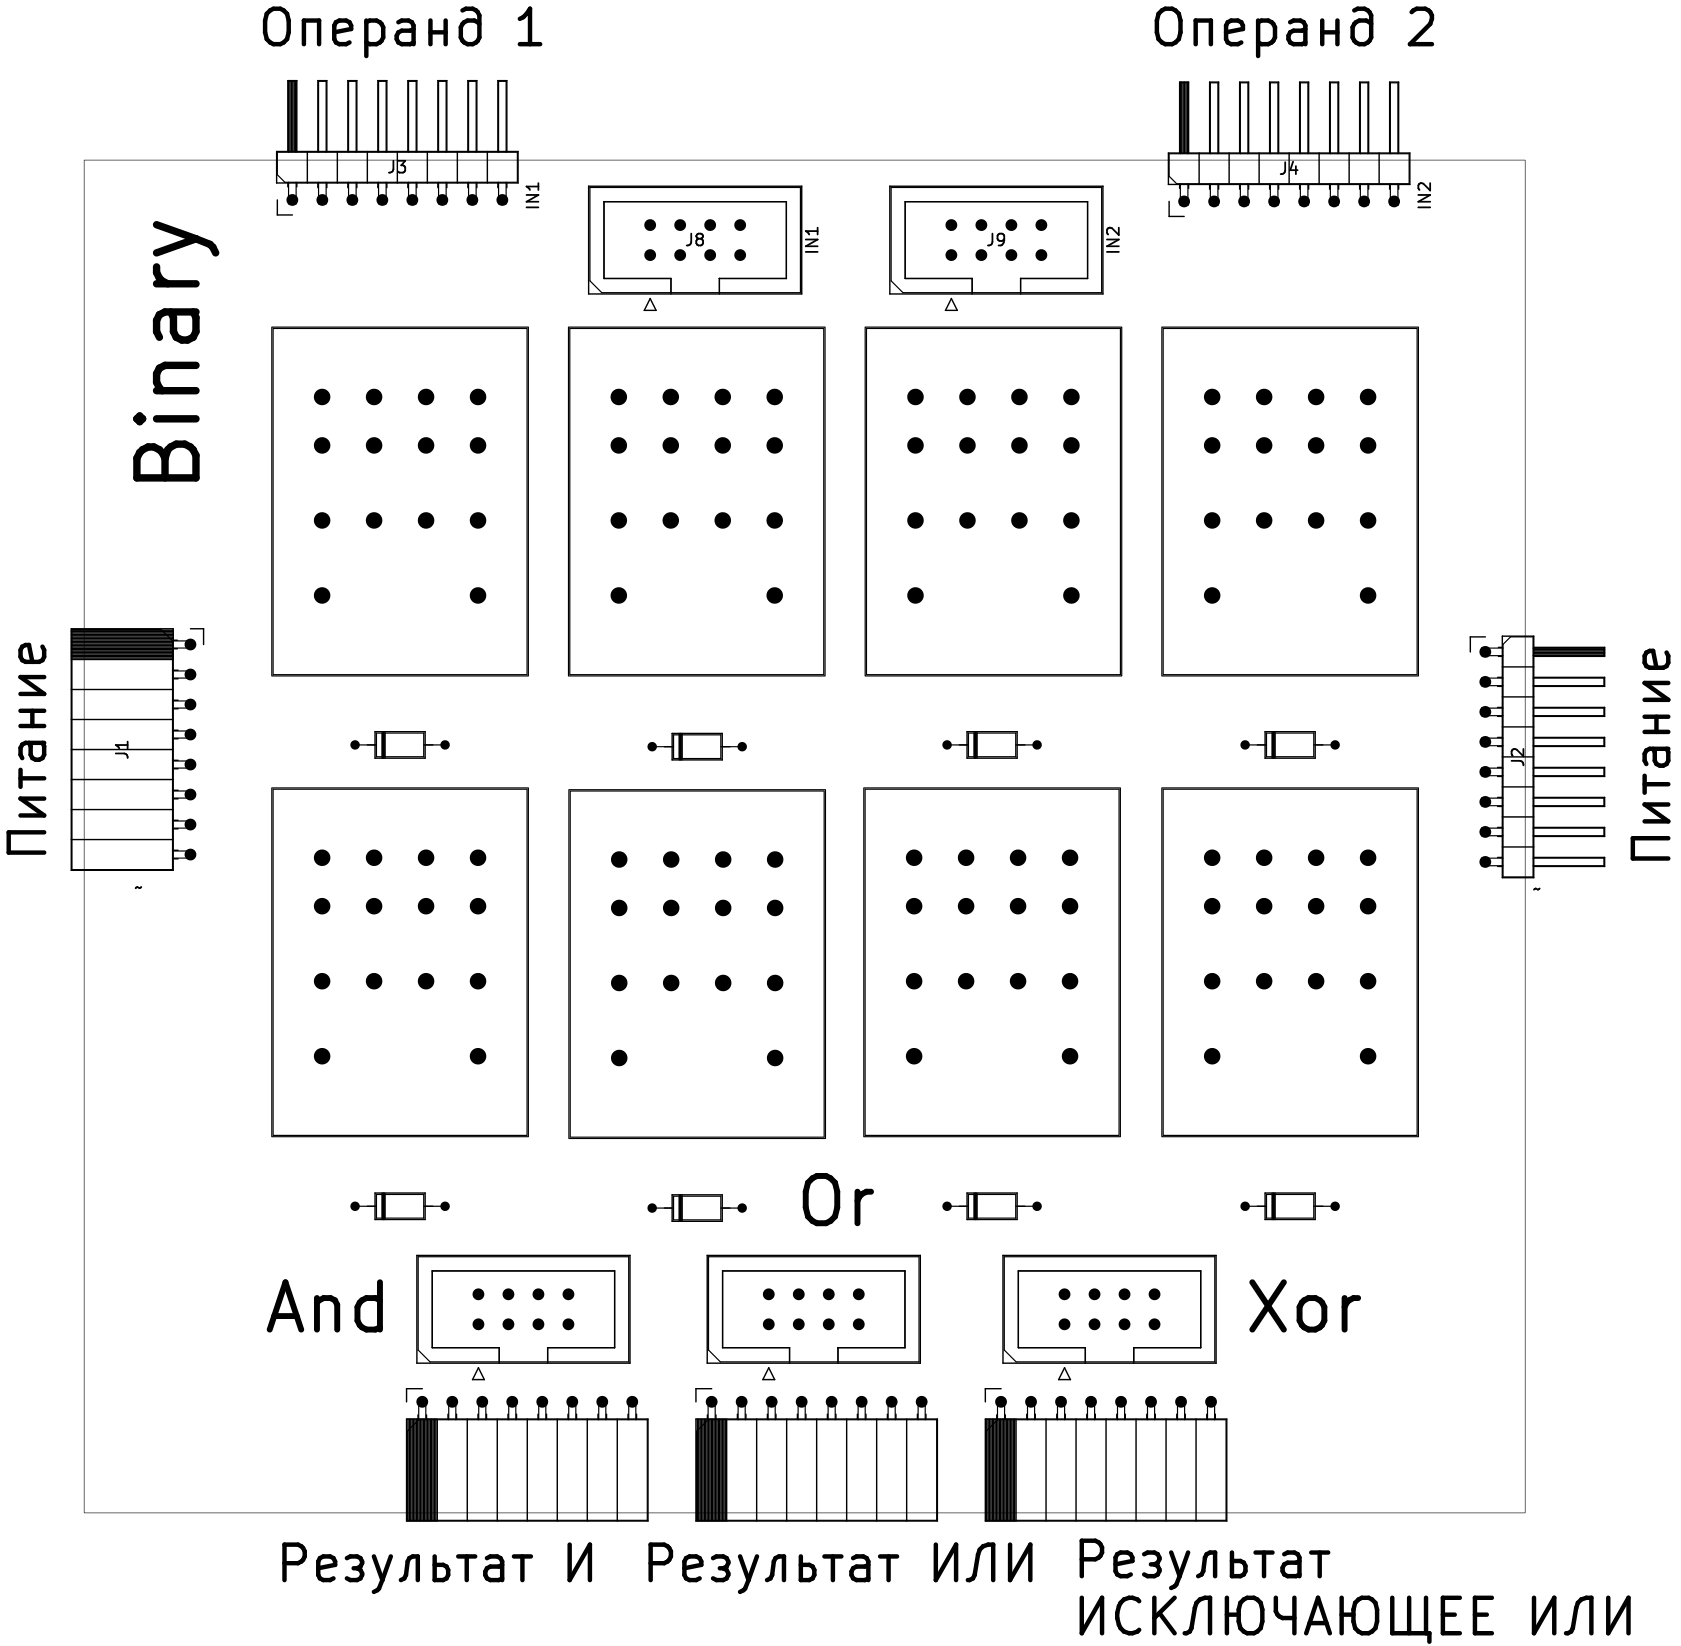
\includegraphics{boards/logic_binary.png}
\end{center}

Модуль логических операций поддерживает вычисление <<И>>, <<ИЛИ>> и <<Исключающее ИЛИ>>.
У модуля есть два четырёхбитных входа и три выхода.
Каждый выход отвечает за одну операцию.

Модуль имеет следующие разъёмы:
\begin{itemize}
  \item Слева и справа: шины для каскадирования нескольких модулей.
        Полезных сигналов через них не передаётся (в отличие от такого же разъёма у модуля унарных операций),
        но можно их использовать для фиксации нескольких логических модулей вместе,
        когда нужны вычисления разрядностью больше четырёх бит.
  \item Сверху: разъёмы для подключения сигналов-операндов.
        Можно подсоединить к шинам, а можно к модулям переключателей или регистрам.
  \item Снизу: три разъёма с выходными сигналами: результатами вычисления
        операций <<И>>, <<ИЛИ>>, <<Исключающее ИЛИ>>.
\end{itemize}


% \subsection{Подготовка}

% \begin{enumerate}
%     \item Как могла бы выглядеть схема для выполнения операцию XOR?
% \end{enumerate}

\section{Практикум}

\subsection{Работа модуля}

Список модулей:
\begin{itemize}
    \item Модуль переключателей: $3$ штуки
    \item Модуль логических операций: $1$ штука
    \item Регистровый модуль: $1$ штука
\end{itemize}


Ко входам модуля подключаются два модуля с тумблерами, а к выходам --- регистр,
куда будет записываться результат.


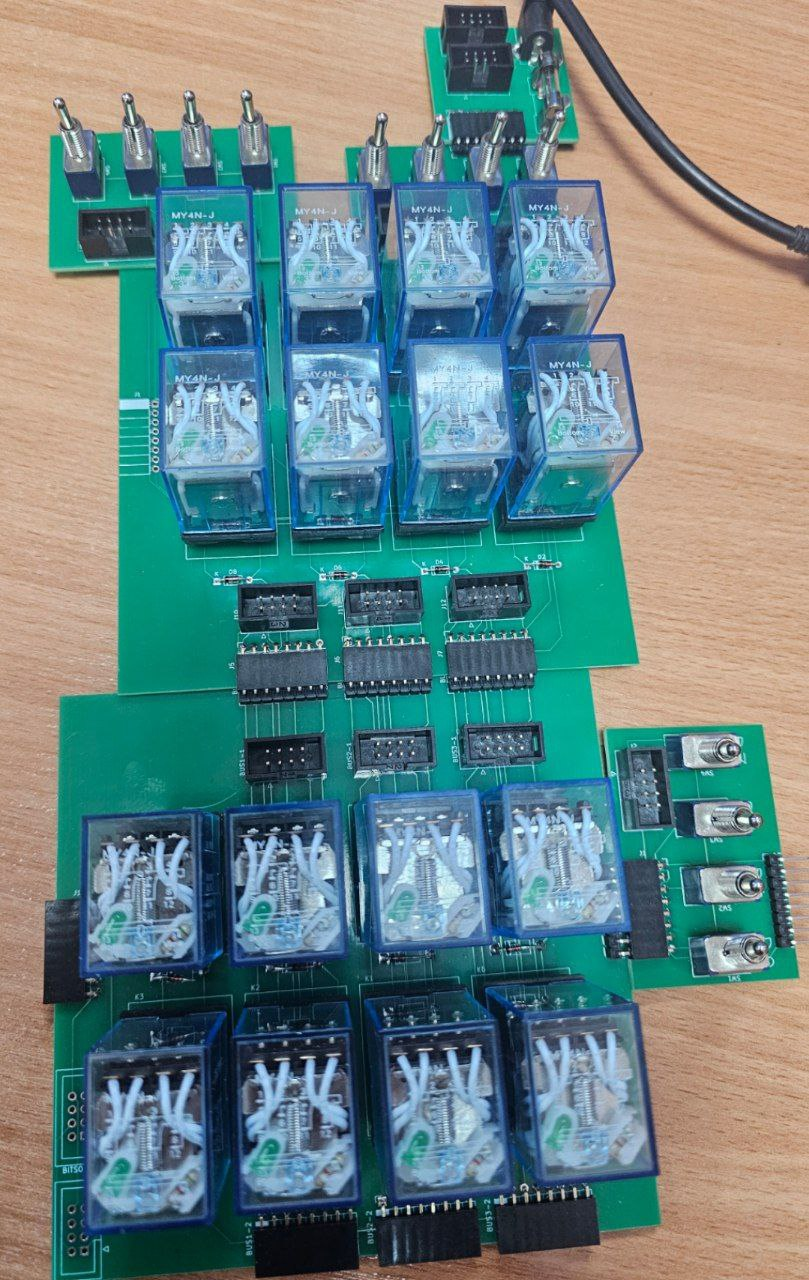
\includegraphics[width=0.5\columnwidth]{photo/logic.jpg}

\begin{enumerate}
    \item Отключите все управляющие сигналы.
    \item Наберите на тумблерах первого операнда значение $1100$.
    \item Наберите на тумблерах второго операнда значение $1010$.
    \item Подключите выходной регистр к шине $1$. Убедитесь, что в него записалось значение $1000$ (AND).
    \item Отключите регистр от шины, сбросьте его значение.
    \item Подключите выходной регистр к шине $2$. Убедитесь, что в него записалось значение $1110$ (OR).
    \item Отключите регистр от шины, сбросьте его значение.
    \item Подключите выходной регистр к шине $3$. Убедитесь, что в него записалось значение $0110$ (XOR).
\end{enumerate}

\section{Задачи}

\begin{enumerate}
    \item Соберите устройство для одновременного вычисления всех трёх логических операций. По сигналу с одного тумблера
          результаты должны записаться в три разных регистра.
\end{enumerate}
